\documentclass[a4paper,12pt]{article}
\usepackage[utf8]{inputenc}
\usepackage[russian]{babel}
\usepackage{amsmath}
\usepackage{amssymb}
\usepackage{enumitem}
\usepackage{graphicx}
\usepackage{hyperref}
\usepackage[a4paper, top= 1cm, bottom=2cm, left=2cm, right=2cm]{geometry}

\hypersetup{
    colorlinks=true,
    linkcolor=blue,
    urlcolor=blue, 
}

\title{Деревья - не только растения}

\begin{document}
\maketitle
    \subsection*{Немного определений}
    \textbf{Дерево} - связный граф без циклов. \\
    \textbf{Лес} - произвольный (не обязательно связный) граф без циклов, проще говоря, это набор из нескольких деревьев.\\ 
    Вершина графа называется \textbf{висячей}, если её степень равна 1.
    \begin{figure}[h]
        \centering
        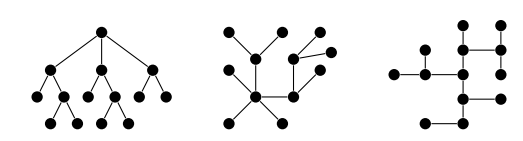
\includegraphics[width=0.5\linewidth]{image.png}
    \end{figure}
    \subsection*{Полезные теоремы}
    \underline{\textbf{Теорема 1.}} Из любого связного графа можно выделить дерево, содержащее все его вершины (остовное дерево); \\
    \textbf{\underline{Теорема 2.}} В связном графе с n вершинами содержится как минимум n − 1 ребро.
    \textbf{\underline{Теорема 3.}} В дереве есть хотя бы одна висячая вершина.
    \subsection*{Задачи}
    \begin{enumerate}
        \item \underline{Упражнение:} Найдите все деревья с пятью вершинами.
        \item В графе все вершины имеют степень равную трём. Докажите, что в графе есть цикл.
        \item Докажите, что граф, в котором каждые две вершины соединены ровно одним простым путем (то есть из каждой вершины можно добраться в любую другую по рёбрам графа только одним способом), является деревом.
        \item Докажите, что при удалении любого ребра из дерева оно превращается в несвязный граф.
        \item Докажите, что связный граф, у которого число рёбер на единицу меньше числа вершин, является деревом.
        \item В некоторой стране 30 городов, причем каждый соединен с каждым дорогой. Какое наибольшее число дорог можно закрыть на ремонт так, чтобы по оставшимся дорогам из каждого города можно было проехать в каждый?
        \item Волейбольная сетка имеет вид прямоугольника размером 50×600 клеток. Какое наибольшее число верёвочек можно перерезать так, чтобы сетка не распалась на куски?
        \item В стране 100 городов, некоторые из которых соединены авиалиниями. Известно, что от каждого города можно долететь до любого другого (возможно, с пересадками). Докажите, что можно побывать во всех городах, совершив не более  а) 198 перёлетов;  б) 196 перелётов.
        \item В стране несколько городов (больше одного); некоторые пары городов соединены дорогами. Известно, что из каждого города можно попасть в любой другой, проезжая по нескольким дорогам. Кроме того, дороги не образуют циклов, то есть если выйти из некоторого города по какой-то дороге и далее двигаться так, чтобы не проходить по одной дороге дважды, то невозможно возвратиться в начальный город. Докажите, что в этой стране найдутся хотя бы два города, каждый из которых соединен дорогой ровно с одним городом.
        \item В стране 15 городов, некоторые из них соединены авиалиниями, принадлежащими трём авиакомпаниям. Известно, что даже если любая из авиакомпаний прекратит полеты, можно будет добраться из каждого в любой другой (возможно, с пересадками), пользуясь рейсами оставшихся двух компаний. Какое наименьшее количество авиалиний может быть в стране?
    \end{enumerate}
\end{document}
